% Options for packages loaded elsewhere
\PassOptionsToPackage{unicode}{hyperref}
\PassOptionsToPackage{hyphens}{url}
%
\documentclass[
]{article}
\usepackage{lmodern}
\usepackage{amssymb,amsmath}
\usepackage{ifxetex,ifluatex}
\ifnum 0\ifxetex 1\fi\ifluatex 1\fi=0 % if pdftex
  \usepackage[T1]{fontenc}
  \usepackage[utf8]{inputenc}
  \usepackage{textcomp} % provide euro and other symbols
\else % if luatex or xetex
  \usepackage{unicode-math}
  \defaultfontfeatures{Scale=MatchLowercase}
  \defaultfontfeatures[\rmfamily]{Ligatures=TeX,Scale=1}
\fi
% Use upquote if available, for straight quotes in verbatim environments
\IfFileExists{upquote.sty}{\usepackage{upquote}}{}
\IfFileExists{microtype.sty}{% use microtype if available
  \usepackage[]{microtype}
  \UseMicrotypeSet[protrusion]{basicmath} % disable protrusion for tt fonts
}{}
\makeatletter
\@ifundefined{KOMAClassName}{% if non-KOMA class
  \IfFileExists{parskip.sty}{%
    \usepackage{parskip}
  }{% else
    \setlength{\parindent}{0pt}
    \setlength{\parskip}{6pt plus 2pt minus 1pt}}
}{% if KOMA class
  \KOMAoptions{parskip=half}}
\makeatother
\usepackage{xcolor}
\IfFileExists{xurl.sty}{\usepackage{xurl}}{} % add URL line breaks if available
\IfFileExists{bookmark.sty}{\usepackage{bookmark}}{\usepackage{hyperref}}
\hypersetup{
  pdftitle={Algorithmic hospital catchment area estimation using label propagation},
  pdfauthor={Rob Challen},
  hidelinks,
  pdfcreator={LaTeX via pandoc}}
\urlstyle{same} % disable monospaced font for URLs
\usepackage[margin=1in]{geometry}
\usepackage{graphicx,grffile}
\makeatletter
\def\maxwidth{\ifdim\Gin@nat@width>\linewidth\linewidth\else\Gin@nat@width\fi}
\def\maxheight{\ifdim\Gin@nat@height>\textheight\textheight\else\Gin@nat@height\fi}
\makeatother
% Scale images if necessary, so that they will not overflow the page
% margins by default, and it is still possible to overwrite the defaults
% using explicit options in \includegraphics[width, height, ...]{}
\setkeys{Gin}{width=\maxwidth,height=\maxheight,keepaspectratio}
% Set default figure placement to htbp
\makeatletter
\def\fps@figure{htbp}
\makeatother
\setlength{\emergencystretch}{3em} % prevent overfull lines
\providecommand{\tightlist}{%
  \setlength{\itemsep}{0pt}\setlength{\parskip}{0pt}}
\setcounter{secnumdepth}{-\maxdimen} % remove section numbering
\usepackage{float} \usepackage{setspace} \doublespacing \floatplacement{figure}{H} \usepackage[ruled,vlined]{algorithm2e}

\title{Algorithmic hospital catchment area estimation using label propagation}
\author{Rob Challen}
\date{}

\begin{document}
\maketitle

Robert Challen\textsuperscript{1,2}; Gareth Griffith\textsuperscript{3};
Lucas Lacasa\textsuperscript{4,5}; Krasimira
Tsaneva-Atanasova\textsuperscript{1,6,7};

\begin{enumerate}
\def\labelenumi{\arabic{enumi})}
\tightlist
\item
  EPSRC Hub for Quantitative Modelling in Healthcare, University of
  Exeter, Exeter, Devon, UK.
\item
  Somerset NHS Foundation Trust, Taunton, Somerset, UK.
\item
  Bristol Medical School, Population Health Sciences, University of
  Bristol, Bristol, UK
\item
  School of Mathematical Sciences, Queen Mary University of London,
  London E1 4NS, UK
\item
  Instituto de Física Interdisciplinar y Sistemas Complejos (IFISC)
  (CSIC-UIB), Campus UIB, 07122, Palma de Mallorca, Spain
\item
  The Alan Turing Institute, British Library, 96 Euston Rd, London NW1
  2DB, UK.
\item
  Data Science Institute, College of Engineering, Mathematics and
  Physical Sciences, University of Exeter, Exeter, UK.
\end{enumerate}

\hypertarget{abstract}{%
\section{Abstract}\label{abstract}}

\emph{\textbf{Background}: Hospital catchment areas define the primary
population of a hospital and are central to assessing the potential
demand on that hospital, for example, due to infectious disease
outbreaks.}

\emph{\textbf{Methods:} We present a novel algorithm, based on label
propagation, for estimating hospital catchment areas, from the capacity
of the hospital and demographics of the nearby population, and without
requiring any data on hospital activity.}

\emph{\textbf{Results:} The algorithm is demonstrated to produce a
mapping from fine grained geographic regions to larger scale catchment
areas, providing contiguous and realistic subdivisions of geographies
relating to a single hospital or to a group of hospitals. In validation
against an alternative approach predicated on activity data gathered
during the COVID-19 outbreak in the UK, the label propagation algorithm
is found to have a high level of agreement and perform at a similar
level of accuracy.}

\emph{\textbf{Conclusions:} The algorithm can be used to make estimates
of hospital catchment areas in new situations where activity data is not
yet available, such as in the early stages of a infections disease
outbreak.}

\hypertarget{introduction}{%
\section{Introduction}\label{introduction}}

During the COVID-19 pandemic, the rapid assessment of the available
capacity of a hospital and the potential demand on its services has been
important in identifying geographical areas where hospital services are
at risk of becoming overwhelmed. Along with epidemic dynamics, residual
hospital capacity guides the imposition of public health measures such
as social distancing. When assessing the load on a hospital due to
COVID-19 the demand may be unevenly distributed in space and rapidly
changing in time. Available capacity may be influenced by multiple
factors, including staff availability. At the same time there may be
fundamental changes to health provision in the acute response of the
pandemic, with for example the cancellation of routine operations. In
the early epidemic in the UK, for example, there was block booking of
private health care providers to assist the NHS (1), and the rapid
creation of large scale field hospitals (2). In previous work we
examined the potential for redirecting patients from one region to
another to balance the load of health care provision (3) and we have
observed this phenomenon as intensive care units reach capacity (4).
When we consider both the change in provision of services and the
redistribution of patients, there is a potential need to redefine the
demographic and geographic profiles of health care service providers
(``catchment areas'' and ``catchment populations'') (5) to allow for
effective planning.

The catchment area or population of a hospital is a broad concept which
serves a number of purposes, such as:

\begin{itemize}
\tightlist
\item
  Definition of the primary population of a hospital (and their
  demographics) for strategic planning purposes (6).
\item
  Definition of higher level organizational structures and collaborative
  networks (7).
\item
  Identification of areas with under, or over provision of services
\item
  Calculation (and visualisation) of incidence and prevalence of disease
  from hospital reported statistics (identifying the denominator) (8)
  and hence admission rates per head of population.
\item
  Preferred routing of patients to hospitals for optimizing specific
  services.
\end{itemize}

There are two general approaches to modelling catchment areas which we
will discuss in detail - activity based or algorithmic approaches.
Algorithmic approaches are based solely on population level information
about regional demographics and hospital capacity. Activity based
approaches minimally require data on hospital activity across all the
region at an individual level, such as individual patient admission
records.

Either of these individual modelling approaches result in a hospital
catchment area that is either overlapping or non-overlapping. An
overlapping output may reflect the fact that patients may have a choice
in the use of the services, and that a range of individually varying
predictors influence individuals' capacity and willingness to adhere to
arbitrarily imposed boundaries. It may also reflect a fundamental
organization of the service, for example the networks of critical care
(4), in which some activity of a hospital caters directly for the local
population, but other activity is conducted supporting other regional
hospitals. As such overlapping approaches may better reflect reality,
but non-overlapping outputs are often a necessary simplification for
secondary analyses, where cross-classification is not specifiable (9).
It is often desirable for secondary analysis that boundaries align with
geographical and organizational boundaries, but non-overlapping outputs
may result in real world cases being incorrectly assigned to a hospital
based on the catchment area, and this will tend to be spatially uneven,
clustering at the fringes of the imposed boundaries (10).

The simplest algorithmic approaches involve straight line distance
weighted to a measure of the size of a hospital (11). This can be
extended by models which use an analogy to gravity to calculate the
potential field of every hospital, based on both capacity (e.g.~beds)
and demand (e.g.~patients) (11--13). The resulting potentials may be cut
off at a specified value, or where they are exceeded by another
hospitals potential, to produce either overlapping or non-overlapping
fields. Such algorithmic approaches may not respect geographical or
existing organizational boundaries, but they can be used to model
hypothetical scenarios, such as the impact of creating a new hospital.
Further details of the range of different models that have been proposed
have been previously published (5,8).

Activity based models began with the proportional flow, or
Norris-Bailey, model (14,15) which examines the proportion of patients
from an area visiting a particular hospital versus the proportion of
patients in an area who visit any health care provider. An extension of
this was recently used to define catchment areas for major injury
following acute trauma (16). More recently modern statistical approaches
have been applied to the same basic activity data including k-Means
classification (8), Bayesian regression modelling. (6) or Markov
Multiscale Community Detection (7,17). Whilst arguably providing a more
accurate reflection of reality, activity based models are predicated on
the availability and recency of activity data, which may exhibit
historical or cultural biases. Depending on the purpose of the catchment
area such historical bias may or may not be desirable (8).

Estimation of hospital catchment areas is a simplification of a complex
logistical and organizational problem. In England, for example, hospital
sites are typically grouped into single organizational units (NHS
trusts) which report combined activity. Thus a single unit of
health-care provision (NHS trust) may have a range of physical
locations, not all of which offer the full range of services. ICU
provision is often focused in a single hospital in an NHS Trust, whereas
acute or step-down beds may be distributed across multiple sites. Some
specialist services, such as intensive care, also may be unevenly
distributed, and larger units used as ``tertiary referral centres''
which take in more complex patients from a wider geographical area.

In the early phase of the COVID-19 pandemic, a rapid estimate was needed
of the potential demand on intensive care services as a result of
observed and forecast infections, in the context of a changing landscape
of health service provision. At this point, there was no comparable data
with which to drive activity based models, and volatile estimates of
hospital capacity. In order to plan provision of additional ventilators
and high dependency beds, we needed a model of geographical catchment
areas that could be used to translate regional epidemiological models of
infections into a prediction of future admissions to individual
hospitals, taking into account the regional demographics, and an
estimate of the expected level of care the patients would need. Such a
catchment area model must interface with existing spatial boundaries
implemented in epidemiological models and publicly available demographic
estimates, and fulfil the following criteria:

\begin{itemize}
\tightlist
\item
  Allow a clean one way mapping from fine grained geographic regions
  (e.g.~from regional demographic estimates or epidemiological models)
  to the coarse grained administrative hospital region.
\item
  Provide contiguous and realistic subdivisions of geographies relating
  to a single hospital or to a hospital group.
\item
  Provide areas that are determined by the capacity of hospital at
  different levels of care provision, and the density of local
  population, or anticipated size of outbreak in the local population.
\item
  Create regions of approximately equal local supply (e.g.~beds) and
  demand (e.g.~patients) at boundaries.
\item
  Respect crude physical geographical boundaries, such as large rivers.
\item
  Flexible in that it can be recomputed rapidly if the background
  parameters change, for example, a regional outbreak or provision of
  additional hospitals, in a way that is not dependant on individual
  level activity data.
\end{itemize}

In this work we present a solution we developed for this problem, and
introduce a novel algorithmic catchment area model which is specifically
designed to meet the needs of the COVID-19 pandemic as described above,
but is globallly applicable to the situation where we can quantify
demand for a resource and a set of point locations that supply that
resource, and could be used, for example, in retail. This model is
inspired by label propagation techniques used for community detection in
networks (18--20). The paper is presented as follows; firstly we
introduce the algorithm, secondly we describe some illustrative
examples, and thirdly we qualitatively compare the output of the
algorithm to both manually created organizational boundaries, and to
observed patient ICU admissions during the first wave of the COVID 19
pandemic.

\hypertarget{materials-and-methods}{%
\section{Materials and Methods}\label{materials-and-methods}}

This section consists of 3 parts: a detailed description of the
algorithmic catchment area model, a description of the data used to
create initial outputs from the model, and a description of initial
assessment of the model against available data.

\hypertarget{algorithm}{%
\subsection{Algorithm}\label{algorithm}}

The algorithm is inspired by label propagation network clustering, where
labels correspond to the supply of a service, and the nodes in the
network correspond to the demand for the service. For illustrative
purposes in this paper we will focus on the example of hospitals, where
the ``supply'' is provision of hospital beds, the ``demand'' is the
population size, and the ``network'' is the neighbourhood of
geographical areas under consideration.

To connect supply and demand, or hospital beds to population size, the
algorithm propagates a number of labels, each representing the source of
supply (e.g.~the hospital), through the geographical network, at a rate
defined by both the size of the supply (e.g.~beds in each hospital), and
the demand for the service (e.g.~the population) within the areas the
label has already propagated to. Thus as demand outstrips supply from a
particular source the rate of label propagation associated with that
source decreases.

We assume the whole geographical region under consideration can be
represented as a mathematical graph, \(G\) and is divided into \(N\)
smaller regions, represented by the vertices \(V\) (where
\(V=V_n, n = 1,2, \dots, N\)) each with known population of size
\(D(V_n)\).

We define \(M\) hospitals located at the geographical points \(P\)
(where \(P = P_m, m = 1,2,3 \dots M\)), and with capacity to supply
\(S(P_m)\) beds. Typically there are fewer hospitals than regions
(\(M<<N\)). We constrain \(P_m\) such that no more than one \(P_m\) is
found within any given \(V\), i.e.~each small region hosts no more than
one hospital. In practice the assumption that a maximum of one hospital
is found in each region is occasionally not true. When this does happen,
we preprocess the data to combine hospitals that are located together
into a single entity.

The connections of neighbouring regions of any area \(V_x\) are defined
by \(E_x = \nu(V_x)\), and likewise the set of neighbouring vertices of
any subgraph \(G_y\) are defined by \(E_y = \nu(G_y)\). These quantities
are readily calculated using the geographical intersection of different
areas and various algorithms exist to calculate these from geo-spatial
data (21,22).

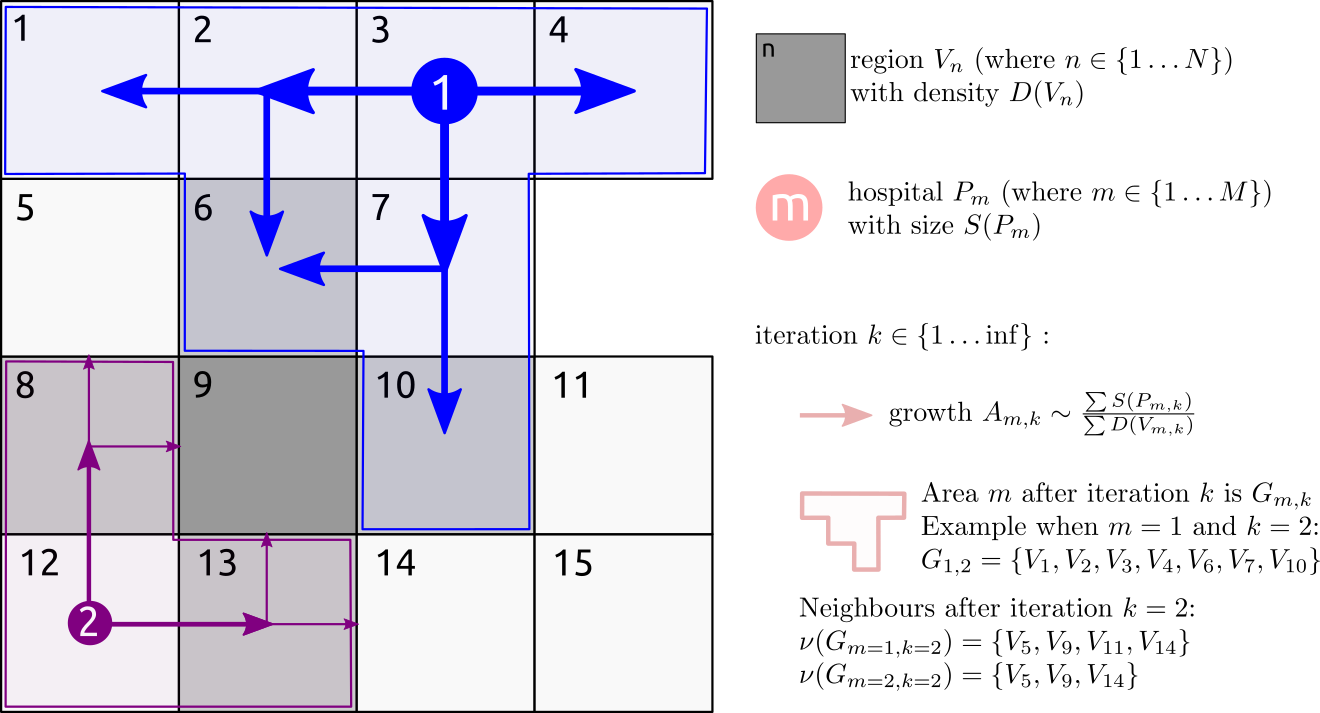
\includegraphics{example.png} Figure 1: Schematic illustration of the
proposed label propagation algorithm. The association of a hospital with
a region propagates from the hospital location (P) into the different
regions (V) at a rate depending on the hospital capacity S(P) and the
population of the region, D(V), at each round of the iteration (k) until
there are no more neighbours to propagate a label to. The direction of
spread is determined by the geographical neighbourhood of each region V

Our goal is to divide the graph \(G\) into \(M\) labelled sub-graphs
\(G_m\) such that the sub-graphs are connected, and that neighbouring
sub-graphs have similar bed availability per unit population
(\(\frac{\sum S_m}{\sum D_m}\)). We do this by assigning a score for
each combination of region and hospital, which is initially zero. For
every iteration of the algorithm this score is incremented in any
unlabelled region that neighbours a region that has been labelled
(i.e.~assigned to a specific hospital). The score is increased by a
small amount determined by the ratio of supply (hospital beds)
available, and demand (population to be served) in the regions assigned
to that hospital. Thus labels propagate more quickly from points with a
high capacity, through regions with a low population density than
vice-versa. The first label to propagate to a given area, and for which
the score is above a threshold is defined as the ``supplier'' for that
area, which is labelled as such. This ensures that each region is served
by only one hospital.

\begin{algorithm}[H]
\setstretch{1.0}
\SetAlgoLined
\SetKwInOut{Input}{Input}
\SetKwInOut{Output}{Output}
\SetKwComment{Comment}{\--- }{}
\Input{$V_N$ - the $N$ regions of demand as a set of geographical polygons}
\Input{$D(V_n)$ - the density of demand in any given region as a function of the region $V_n$}
\Input{$P_M$ - a set of $M$ labelled suppliers as a set of geographical points}
\Input{$S(P_m)$ - the capacity of supply at any given supply point as a function of the supplier $P_m$}
\Input{$C_{growth}$ - a rate constant defining rate of label propagation}
\Output{$G_M$ - $M$ labelled subgraphs of graph $G$, relating to the catchment areas of suppliers $P_M$}
\BlankLine
\Comment{define $G$ as the graph consisting of geographical regions $V_N$, connected by edges, $E_N$, given by their geographical neighbours $\nu(V_N)$:}
$E_N \gets \nu(V_N)$\;
$G \gets (V_N, E_N)$\;
\Comment{define $V_M$ and $V^{new}_{M,0}$ as the geographic regions of $G$ serviced by points $P_M$, and $G_{M,0}$ as a set of labelled sub-graphs (also initially consisting solely of the vertices $V_M$):}
$V_M \gets G \cap P_M$\;
$V^{new}_{M,0} \gets V_M$;
$G_{M,0} \gets V_M$\;
\Comment{define the initial unlabelled set of vertices:}
$U_0 \gets \neg V_{M}$\;
\Comment{define the initial un-labelled neighbours of labelled sub-graphs, $G_M$:}
$U_{M,0} \gets \nu(V_M)$\;
\Comment{define an accumulated growth score for each un-labelled neighbour $U_{M,0}$ of each $G_{M,0}$:}
$A_{U_{M,0}} \gets 0$\;
\BlankLine
$k \gets 0$\;
\Comment{execute the loop while there are still unlabelled vertices and there exist some unlabelled neighbours of labelled vertices}
\While{$|U_k| > 0$ and $|U_{M,k}| > 0$} {
  $k \gets k+1$\;
  \BlankLine
  \Comment{define the un-labelled vertices as the set of $V$ not contained in any of $G_{M,k-1}$:}
  $U_k \gets \neg G_{M,k-1}$\;
  \Comment{define the un-labelled neighbours of $G_{M,k-1}$ as $U_{M,k}$ as the previously unlabelled neighbours and the neighbours of the most recently labelled neighbours $V^{new}_{M,k-1}$:}
  $U_{M,k} \gets U_{M,k-1} \cup (U_k \cap \nu(V^{new}_{M,k-1}))$\;
  \Comment{define the reserve capacity, $R_M$, to supply existing labelled, $G_{M,k-1}$,  and un-labelled neighbours $U_{M,k}$, as:}
  $R_M \gets \frac{S(P_M)}{D(U_{M,k} \cup G_{M,k-1})}$\;
  \Comment{for unlabelled areas only, update the accumulated growth score, $A_{U_{M,k}}$, with the normalised rank of the reserve capacity and multiplied by a constant $C_{growth} > 1$ representing the speed at which the accumulated growth score increases in all areas:}
  $R_{M,k} \gets R_m \{m \in U_{M,k}\}$\;
  $A_{U_{M,k}} \gets A_{U_{M,k-1}} + C_{growth} \times \text{rank}(R_{M,k})/|R_{M,k}|$\;
  \Comment{for all the un-labelled vertices, select the label $M$, with the highest score, and if the accumulated score has reached the threshold of 1, incorporate it into the labelled sub-graph, $G_{M,k-1}$:}
  $A^{max}_{U_k} = \text{max}(A_{U_{m,k}},m \in M)$\;
  $V^{new}_{M,k} \gets U_{M,k} \in \{A^{max}_{U_k} > 1\}$\;
  $G_{M,k} \gets G_{M,k-1} \cup V^{new}_{M,k}$\;
  $U_{M,k+1} \gets U_{M,k} \cap \neg V^{new}_{M,k}$\;
}
\Return{$G_{M,k}$}
\caption{A weighted label propagation algorithm for matching geographical supply to demand}
\end{algorithm} 

\hypertarget{qualitative-testing-data}{%
\subsection{Qualitative testing data}\label{qualitative-testing-data}}

The algorithm requires firstly an estimate of demand, for this we used
population counts, secondly a geographical network and thirdly an
estimate of supply, in this case hospital capacity data.

For the UK there are detailed estimates of the population at granular
geographic detail (lower super output area - LSOA) available from the
Office of National Statistics (ONS) for England and Wales, and the
National Records Service (NRS) in Scotland (23,24). These population
estimates are available by single year of age for each area. These are
combined to create a single figure for the adult population of each
small geographic area.

Each geographical area is associated with a boundary file also provided
by the ONS and NRS (25,26).

To estimate the capacity of hospitals we used a range of primary sources
(described in the supplementary materials) to manually compile a list of
NHS and independent hospital sites. When not provided in the primary
sources, we identified their geographical locations from their postcode,
and we estimated bed numbers from both a combination of published NHS
statistics and from daily COVID-19 situation reports from early April
2020, provided by the NHS. The situation reports detailed both available
beds at this point in time but also gave an indication of maximum surge
capacity for high dependency beds. These data were manually curated and
are indicative of the state of the NHS at maximal readiness. Bed state
estimates for independent hospital providers were also available through
the situation reports.

In Northern Ireland, population estimates were not available at a
similar geographical resolution as the ONS and NRS sources, and we are
unaware of any publicly available hospital capacity estimates. They were
therefore not included in this analysis.

The detail of the original data sources we used is presented in the
supplementary material, not all of which are publicly available. The
algorithm is implemented as an R package \texttt{arear} (available from
\url{https://terminological.github.io/arear/}), which also contains both
the manually curated hospital capacity and data pertaining derived
demographics data described here.

\hypertarget{validation}{%
\subsection{Validation}\label{validation}}

There is no ground truth for the catchment areas for hospitals in the
NHS during the COVID-19 pandemic. The rationale for original development
of this algorithm was to make an estimate in absence of any activity
data, in the early stages of the pandemic. Since then activity data has
become available and this allows us to validate the label propagation
approach to the activity based approach.

The activity based mapping takes the form of a many-to-many
probabilistic mapping between lower tier local authority districts
(LTLA) and NHS Acute Trusts in England derived from Secondary Uses
Service (SUS) health-care data for England (27). We create equivalent
probabilistic associations between the coarse grained LTLA and NHS
trusts by generating a fine grained lower super output area (LSOA)
catchment area for NHS trusts using the label propagation algorithm, and
the demographic and bed capacity estimates described above. This is
aggregated to coarse grained local authority districts using mapping
files provided by the ONS (28), weighted by LSOA population size (23)
(Source: Office for National Statistics licensed under the Open
Government Licence v.3.0). This equivalent mapping based on the label
propagation algorithm is compared to the activity based mapping
graphically. The expected number of admissions to each NHS trust from
each LTLA, based on LTLA population size, and estimated using each
method compared with the intra-class correlation coefficient (29,30)
using a mean-of-raters, absolute-agreement, two-way random-effects
model(31), as implemented in the R package \texttt{irr}(32).

Secondly we obtain the coarse location (partial UK postcode, also known
as outcode) from a list of intensive care patients admitted between 20th
October 2000 and 16th March 2021 from the CHESS data set (33), which is
an anonymised patient level hospital admission data set. We use outcode
boundary shapes (34), LSOA demographic estimates, and an areal
interpolation (35) to generate an estimate of demographics for each
outcode. Using this outcode based regional population estimate, outcode
boundary shapes, and the manually curated high dependency unit capacity
estimates we calculate an outcode based catchment area estimate from
which we are able to predict the NHS trust each patient was admitted to
based on their outcode, which we compare to the observed NHS trust from
the CHESS data. For this comparison we calculate both the multinomial
accuracy, and for each NHS trust, the one-versus-all binomial accuracy
as follows:

\[
\text{accuracy} = \frac{1}{|X|} \sum_{k \in G} \sum_{g_{obs}(x) = k} I \left(g_{pred}(x) = g_{obs}(x)\right)
\] where \(X\) is the set of observations, \(G\) is the set of NHS
trusts, \(g_{pred}\) and \(g_{obs}\) are the predicted and observed
classes respectively and \(I\) is the indicator function which returns
\(1\) if the predicted match observed and \(0\) otherwise.

For the activity based approach we assign each patient to a LTLA by
virtue of the geographical location of the centroid of their outcode
shape and then determine the most probable NHS trust associated with
that LTLA. This forms a prediction of the NHS trust based on the
patient's outcode, which we can compare to the observed NHS trust in the
same manner as above.

\hypertarget{results}{%
\section{Results}\label{results}}

\hypertarget{qualitative-testing-results}{%
\subsection{Qualitative testing
results}\label{qualitative-testing-results}}

The results presented in this section qualitatively test the algorithm
to determine whether it is producing catchment area regions that are
geographically contiguous, aligned with existing demographic boundaries,
respect coarse geographical boundaries such as large rivers. The
catchment areas should also produce estimates that minimise differences
in the level of service provision from area to area, and we expect the
overall regional variation of supply versus demand to be locally smooth.
Figure 2 shows a catchment area based on individual hospitals that
offered high dependency beds during April 2020, and a regional demand
based on population estimates of adults in lower super output areas. The
resulting set of catchment areas presented in panel A and C behave as
desired in terms of the geographical properties. They also produce a
fairly uniform density of high dependency bed provision per capita
population, from region to region, as seen in panel B. In areas where
there are high densities of hospitals such as London where the
algorithm, by design, cannot propagate from centrally located hospitals
past more peripheral hospitals, leading to small numbers of areas with
high provision per head of population. This is discussed further below.

\begin{center}\includegraphics{/home/terminological/Dropbox/covid19/catchment-areas/HDU_UK_example} \end{center}

Figure 2: Panels A and C show a LSOA based catchment area map estimated
from the high dependency bed state in the UK in early April 2020, with
catchment area boundaries shown in white. Red circles are NHS hospital
sites with high dependency capacity. Map source: Office for National
Statistics licensed under the Open Government Licence v.3.0, Contains OS
data © Crown copyright and database right 2020. Panel B shows the
distribution of high dependency beds per 100K population for each of the
catchment areas defined by the algorithm.

Further qualitative investigation of the properties of the algorithm are
shown in Figure 3 where we see more regional detail of the same
algorithm applied this time to general hospital beds rather than high
dependency beds. Panel A shows the boundaries of the estimated catchment
areas in white against the population density of a small area of the
South West of England containing three hospitals (Plymouth, Torbay and
the Royal Devon and Exeter hospitals). We can see in this example the
extent of the catchment area to the South of Torbay is defined by the
Dart river estuary, thus respecting such geographical boundaries.

Figure 3 panel B shows details about the progression of the algorithm
from one iteration to the next, as labels propagate from each of the
hospitals into the surrounding areas until encountering another
catchment area. As we expect from the design the algorithm is seen to
spread from hospital sites quickly through areas of low population
density (panel A), such as the countryside surrounding Plymouth in the
bottom left, and more slowly through areas of higher population density
such as the areas surrounding Torbay in the middle right.

\begin{center}\includegraphics{/home/terminological/Dropbox/covid19/catchment-areas/HDU_Acute_SW_example} \end{center}

Figure 3: Detail LSOA based catchment area map for NHS trusts estimated
from the general hospital bed states in the UK in early April 2020. Red
circles are NHS hospital sites. In panel A the fill represents a
relative measure of regional population density, with yellow areas being
high density in and around cities. In Panel B the same areas are shown
but this time the fill shows the iteration number at which the algorithm
labelled a specific area, and the propagation of the algorithm by
arrows. Map source: Office for National Statistics licensed under the
Open Government Licence v.3.0, Contains OS data © Crown copyright and
database right 2020

\hypertarget{validation-1}{%
\subsection{Validation}\label{validation-1}}

In comparing the label propagation mapping to the activity based mapping
we see that the proportions of any given LTLA that are assigned to any
given trust are similar between the two methods (Figure 4, panel A) with
a clear trend to agreement. The major differences are seen in the
extremes where, for example, in the top left of panel A, the activity
based approach may predict that no patients are observed in a given
hospital from a given LTLA, whereas the label propagation approach
predicts the opposite. Panel B shows the same relationship but this time
scaled by the population size in each area, and this shows that the
impact of differences between predictions seen in panel A is in areas
with smaller populations and is therefore attenuated. Calculation of the
intra-class correlation coefficient between the predicted number of
cases from each method gives excellent agreement between the two
methods, with a value of 0.94 (95\% CI: 0.93 -- 0.95) using a
mean-of-raters, absolute-agreement, two-way random-effects model(31).

\begin{center}\includegraphics{/home/terminological/Dropbox/covid19/catchment-areas/prob_comparison_agreement} \end{center}

Figure 4: Classification agreement between activity based approach and
label propagation algorithm. Each point is a unique combination of lower
tier local authority and NHS trust and in panel A the proportion of the
LTLA assigned to that trust is plotted for the activity based algorithm
on the x-axis and the label propagation algorithm on the y-axis. In
panel B the total number of cases assigned to each trust is plotted when
the population size for the area is considered. The blue line represents
perfect agreement.

In Figure 5 we compare observed admissions to ITU to predictions made by
the label propagation algorithm and the activity based approach. As
there are 178 trusts under consideration which form a large number of
distractors for each prediction, a low value for the multinomial
accuracy could be expected. The overall accuracy of both methods is
comparable at 72.6\%---72.4\%. The distribution of the binomial
one-versus-all accuracy in the histogram shows that the prediction
performance is better for some trusts than others, and that the accuracy
of the activity based approach has greater variability than that of the
label propagation approach. Across the whole country exact agreement
between the observed location of hospital admission and the predicted
location of hospital admission based on the label propagation catchment
area was seen in 12534 out of 17274 cases, and the Matthew's correlation
coefficient was 0.72.

\begin{center}\includegraphics{/home/terminological/Dropbox/covid19/catchment-areas/sari_accuracy_comparison} \end{center}

Figure 5: Accuracy measures for the predictions of activity based and
label propagation approaches based on UK postcode outcodes, and a subset
of observed NHS trust of intensive care admissions in England between
20th October 2000 and 16th March 2021. The histogram shows the
distribution of the balanced accuracy for each NHS trust in a one-vs-all
binomial evaluation, and the inset table shows the overall accuracy from
the multinomial evaluation, along with the raw counts af overall
evaluations and correct predictions for each method

In Table 1 we qualitatively examine the ten NHS Trusts that have the
highest number of ITU patients that the label propagation algorithm
predicted to be admitted elsewhere, and mis-classified them. These
represent 1833 (38.7\%) of the total mis-classifications. The majority
of these 10 hospitals are major tertiary referral intensive care units,
or specialist centres, as demonstrated by them being in the top 10
centile of NHS trusts by ITU bed capacity. This result is consistent
with both the possibilities that severely ill patients may end up in
specialist centres rather than their closest hospital for treatment, or
that in the event of a large surge in cases, patients may overflow from
smaller to larger intensive care units. Both of these could lead to
mis-classification of these patients by the label propagation algorithm,
as we see here.

Table 1: The NHS trusts with the ten most misclassified covid ITU cases
as assigned by the label propagation algorithm

\begin{center}\includegraphics{/home/terminological/Dropbox/covid19/catchment-areas/Non_matching_trusts} \end{center}

\hypertarget{discussion}{%
\section{Discussion}\label{discussion}}

We have presented an algorithm for rapidly estimating hospital catchment
areas for use when activity data is not available. We demonstrate how
the output responds to the different capacities of the different levels
of care provided (e.g.~high dependency versus general hospital beds). We
present catchment areas calculated using population size as demand, and
total hospital beds as supply. This algorithm may be useful for longer
term strategic planning, but was conceptualized as part of an acute
response to COVID-19 outbreak. In this case we can use the different
parameters for demand, for example local COVID-19 infection prevalence,
and different parameters for supply, for example availability to staffed
hospital beds. Our approach is novel in that it allows adaptation of
local service provision to predictions of disease prevalence from
epidemiological models of COVID-19 and real time bed states provided by
NHS trusts. This allows us to model the degree of elasticity in the
system to absorb localised shocks, caused by regional outbreaks, it
helps us to develop a better concept of when services are being at risk
of becoming overwhelmed, and allow routing of new admissions away from
overloaded hospitals.

Benchmarking our algorithm against activity based approaches produced
good to excellent agreement and application to both methods to real
world patient admission data produces a very similar result. The finding
that naive application of our algorithm to real world patient admission
classifies only 72.6\% correctly is explained by two things, firstly
accuracy at boundaries decreases as the number of boundaries increases
(10) and secondly the fact that many of the top 10 mis-classified trusts
are major tertiary referral centres, which may take patients from
distant regions for specialist care. This suggests that our constraint
that catchment areas should be non overlapping is not borne out in
reality for these cases.

Overlapping catchment areas could be modeled by multiple layers of
non-overlapping catchment areas. When we consider the provision of
intensive care services in the UK during COVID-19, we propose there are
at least 3 layers of hospital service provision: there is a local
service, which provides care for patients from nearby. A subset of
hospitals additionally provide a regional, or tertiary referral, service
layer which takes sicker patients from neighbouring hospitals in larger
areas. The final layer is a crisis overflow layer provided by the NHS
Nightingale field hospitals (2). Each of these layers may be considered
to have somewhat independent catchment areas. We propose that dividing
the larger hospitals into local and regional services and considering
the tertiary referral network as a second layer, with its own larger
catchment area would improve the performance of the algorithm against
real activity data. In such a layered model of catchment areas there is
interplay between local layer demand for hospital beds and capacity for
regional tertiary care provision, which will dynamically affect the
``catchment area'' for regional tertiary care provision, potentially on
a day to day basis. In previous work we looked at the opportunities for
balancing the load between different hospitals (3) when transferring
COVID-19 patients away from overloaded areas, however moving unwell
patients between hospitals is ideally minimized. With this algorithm we
enable the dynamic re-specification of local service catchment areas and
hospital tertiary referral networks, based on evolving demand. Coupled
with flexible load sharing has interesting potential to model or
influence patient admissions around the whole hospital network.

Hospital capacity is difficult to accurately estimate. During this work
we encountered many of the uncertainties that influence capacity. The
ability of a hospital to provide a bed to a patient depends on a
multitude of factors, including staff availability, which may vary
during the different stages of the pandemic. The ability of hospitals to
absorb large numbers of emergency patients by re-configuring their
service provision (e.g canceling routine operations) and providing
overflow or ``surge'' high dependency capacity for short periods of time
makes putting a single number on hospital capacity difficult. The
ability to recalculate catchment areas based on changing assumptions
around capacity is a strength of our approach, and in the future could
be used to analyse the impact of introducing new capacity into the
hospital system. One further limitation to note is that the algorithm
does not consider travel time between regions which may increase both as
the geographical size increases but also as the population density
increases due to traffic and form a barrier to patients accessing
services. Adding a travel time penalty to the rate of label spread into
the model is possible given some estimate of the ease of transport
within and between regions, and this is an area of future work.

There are opportunities to extend our algorithm. The general approach of
label propagation in networks has been more widely studied and newer
approaches described (19,36,37) which allow overlapping communities.
This may address some of the issues described above. These are appealing
and a possible avenue for future extension of the algorithm. There
persists however an open question about whether the overlapping nature
of hospital service provision observed in activity data is not really a
reflection of patient choice, but actually the result of subtly
different services, or different levels of service, being provided by
different hospitals to different catchment areas. Thus a specialist
cancer hospital close to a specialist paediatric hospital will have
geographically overlapping catchment areas, but in reality these
hospitals are not providing the same service to the same population.
This line of argument suggests that the concept of a single overlapping
hospital catchment area is also an over-simplificiation, and when we
take into account the heterogeneity of different services offered by a
hospital, we propose that a hospital's overall catchment area may be
well modeled by a collection of non-overlapping catchment layers.

\hypertarget{conclusions}{%
\section{Conclusions}\label{conclusions}}

This label propagation algorithm for estimating hospital catchment areas
is a pragmatic solution to determining geographical and demographic
subsets of the population when there is no previous activity data
available. It suits situations where the level of service provision and
demand on the hospital system is dynamic, as has been the case in the
COVID-19 pandemic. The algorithm is simple and satisfies the major
criteria we set out in the introduction, in that it provides a mapping
from low level geographic regions which provide contiguous and realistic
subdivisions of geographies relating to a single hospital or to a group
of hospitals. The areas are determined by the capacity of the hospital
and the density of local population, and are approximately equal in
terms of local supply (e.g.~beds) and demand (e.g.~patients) at
boundaries.

The algorithm depends solely on data reflecting supply and geographical
demand for a service, and as such is quite generic and potentially more
widely applicable outside of healthcare. Although we have discussed
catchment areas in terms of the capacity of hospital beds, and demand of
local populations, there is nothing to prevent us defining capacity in
any other way - a heuristic on staffing levels may be appropriate, or in
different contexts, availability of medical imaging devices. Likewise,
demand may be refined to reflect sub-populations at risk of disease, or
may even be the output of a predictive model. As such our approach is
applicable to a wide variety of problems.

\hypertarget{references}{%
\section{References}\label{references}}

\hypertarget{refs}{}
\leavevmode\hypertarget{ref-CoronavirusThousandsExtra2020}{}%
1. Coronavirus: Thousands of extra hospital beds and staff. BBC News: UK
{[}Internet{]}. 2020 Mar 21 {[}cited 2020 Dec 16{]}; Available from:
\url{https://www.bbc.com/news/uk-51989183}

\leavevmode\hypertarget{ref-CoronavirusNightingaleHospital2020}{}%
2. Coronavirus: Nightingale Hospital opens at London's ExCel centre. BBC
News: UK {[}Internet{]}. 2020 Apr 3 {[}cited 2020 Dec 17{]}; Available
from: \url{https://www.bbc.com/news/uk-52150598}

\leavevmode\hypertarget{ref-lacasaFlexibleMethodOptimising2020}{}%
3. Lacasa L, Challen R, Brooks-Pollock E, Danon L. A flexible method for
optimising sharing of healthcare resources and demand in the context of
the COVID-19 pandemic. PLOS ONE. 2020 Oct 21;15(10):e0241027.

\leavevmode\hypertarget{ref-pettCriticalCareTransfers2020}{}%
4. Pett E, Leung HL, Taylor E, Chong MSF, Hla TTW, Sartori G, et al.
Critical care transfers and COVID-19: Managing capacity challenges
through critical care networks. Journal of the Intensive Care Society.
2020 Dec 16;1751143720980270.

\leavevmode\hypertarget{ref-jonesModellingCatchmentAreas2011}{}%
5. Jones S, Wardlaw J, Crouch S, Carolan M. Modelling catchment areas
for secondary care providers: A case study. Health Care Manag Sci. 2011
Sep;14(3):253--61.

\leavevmode\hypertarget{ref-wangCatchmentAreaAnalysis2015}{}%
6. Wang A, Wheeler DC. Catchment Area Analysis Using Bayesian Regression
Modeling. Cancer Inform. 2015 Jan 1;14s2:CIN.S17297.

\leavevmode\hypertarget{ref-clarkeDefiningHospitalCatchment2019}{}%
7. Clarke JM, Barahona M, Darzi AW. Defining Hospital Catchment Areas
Using Multiscale Community Detection: A Case Study for Planned
Orthopaedic Care in England. bioRxiv. 2019 May 3;619692.

\leavevmode\hypertarget{ref-gilmourIdentificationHospitalCatchment2010}{}%
8. Gilmour SJ. Identification of Hospital Catchment Areas Using
Clustering: An Example from the NHS. Health Services Research.
2010;45(2):497--513.

\leavevmode\hypertarget{ref-jonesEthnicResidentialSegregation2015}{}%
9. Jones K, Johnston R, Manley D, Owen D, Charlton C. Ethnic Residential
Segregation: A Multilevel, Multigroup, Multiscale Approach Exemplified
by London in 2011. Demography. 2015 Dec 1;52(6):1995--2019.

\leavevmode\hypertarget{ref-arcayaAreaVariationsHealth2012}{}%
10. Arcaya M, Brewster M, Zigler CM, Subramanian SV. Area variations in
health: A spatial multilevel modeling approach. Health Place. 2012
Jul;18(4):824--31.

\leavevmode\hypertarget{ref-reillyLawRetailGravitation1931}{}%
11. Reilly WJ. The law of retail gravitation, New York: W.J. Reilly;
1931.

\leavevmode\hypertarget{ref-huffDefiningEstimatingTrading1964}{}%
12. Huff DL. Defining and Estimating a Trading Area. Journal of
Marketing. 1964 Jul 1;28(3):34--8.

\leavevmode\hypertarget{ref-stewartInverseDistanceVariation1941}{}%
13. Stewart JQ. An Inverse Distance Variation for Certain Social
Influences. Science. 1941 Jan 24;93(2404):89--90.

\leavevmode\hypertarget{ref-baileyStatisticsHospitalPlanning1956}{}%
14. Bailey NTJ. Statistics in Hospital Planning and Design. Journal of
the Royal Statistical Society: Series C (Applied Statistics).
1956;5(3):146--57.

\leavevmode\hypertarget{ref-norrisRoleStatisticsRegional1952}{}%
15. Norris V. Role of Statistics in Regional Hospital Planning. Br Med J
{[}Internet{]}. 1952 Jan 19 {[}cited 2020 Dec 17{]};1(4750):129--33.
Available from:
\url{https://www.ncbi.nlm.nih.gov/pmc/articles/PMC2022292/}

\leavevmode\hypertarget{ref-alexandrescuProposedApproachDefining2008}{}%
16. Alexandrescu R, O'Brien SJ, Lyons RA, Lecky FE, Trauma Audit,
esearch Network. A proposed approach in defining population-based rates
of major injury from a trauma registry dataset: Delineation of hospital
catchment areas (I). BMC Health Serv Res. 2008 Apr 10;8(1):80.

\leavevmode\hypertarget{ref-clarkeIdentifyingNaturallyOccurring2020}{}%
17. Clarke J, Beaney T, Majeed A, Darzi A, Barahona M. Identifying
naturally occurring communities of primary care providers in the English
National Health Service in London. BMJ Open. 2020 Jul 1;10(7):e036504.

\leavevmode\hypertarget{ref-fortunatoCommunityDetectionNetworks2016}{}%
18. Fortunato S, Hric D. Community detection in networks: A user guide.
Physics Reports. 2016 Nov 11;659:1--44.

\leavevmode\hypertarget{ref-xieCommunityDetectionUsing2011}{}%
19. Xie J, Szymanski BK. Community detection using a neighborhood
strength driven Label Propagation Algorithm. In: 2011 IEEE Network
Science Workshop. 2011. pp. 188--95.

\leavevmode\hypertarget{ref-xieLabelRankStabilizedLabel2013}{}%
20. Xie J, Szymanski BK. LabelRank: A stabilized label propagation
algorithm for community detection in networks. In: 2013 IEEE 2nd Network
Science Workshop (NSW). 2013. pp. 138--43.

\leavevmode\hypertarget{ref-bivandRgeosInterfaceGeometry2020}{}%
21. Bivand R, Rundel C, Pebesma E, Stuetz R, Hufthammer KO, Giraudoux P,
et al. Rgeos: Interface to Geometry Engine - Open Source ('GEOS')
{[}Internet{]}. 2020 {[}cited 2020 Dec 18{]}. Available from:
\url{https://CRAN.R-project.org/package=rgeos}

\leavevmode\hypertarget{ref-pebesmaSimpleFeaturesStandardized2018}{}%
22. Pebesma E. Simple Features for R: Standardized Support for Spatial
Vector Data. The R Journal {[}Internet{]}. 2018 {[}cited 2020 Dec
18{]};10(1):439--46. Available from:
\url{https://journal.r-project.org/archive/2018/RJ-2018-009/index.html}

\leavevmode\hypertarget{ref-PopulationEstimatesOffice}{}%
23. Population estimates - Office for National Statistics
{[}Internet{]}. {[}cited 2020 Nov 17{]}. Available from:
\url{https://www.ons.gov.uk/peoplepopulationandcommunity/populationandmigration/populationestimates}

\leavevmode\hypertarget{ref-teamNationalRecordsScotland2013}{}%
24. Scotland Web Team NR of. National Records of Scotland
{[}Internet{]}. National Records of Scotland; National Records of
Scotland; 2013 {[}cited 2020 Dec 7{]}. Available from:
\url{/statistics-and-data/statistics/statistics-by-theme/population/population-estimates/2011-based-special-area-population-estimates/small-area-population-estimates/time-series}

\leavevmode\hypertarget{ref-OpenGeographyPortal}{}%
25. Open Geography Portal {[}Internet{]}. {[}cited 2020 Nov 17{]}.
Available from: \url{https://geoportal.statistics.gov.uk/}

\leavevmode\hypertarget{ref-spatialdata.gov.scotDataZoneBoundaries2020}{}%
26. SpatialData.gov.scot SG. Data Zone Boundaries 2011 {[}Internet{]}.
2020 {[}cited 2020 Dec 7{]}. Available from:
\url{https://data.gov.uk/dataset/ab9f1f20-3b7f-4efa-9bd2-239acf63b540/data-zone-boundaries-2011}

\leavevmode\hypertarget{ref-meakinNHSTrustLevel2021}{}%
27. Meakin S, Abbott S, Funk S. NHS trust level Covid-19 data aggregated
to a range of spatial scales. 2021.

\leavevmode\hypertarget{ref-officeofnationalstatisticsLowerLayerSuper}{}%
28. Lower Layer Super Output Area (2011) to Ward (2019) Lookup in
England and Wales - Office for National Statistics {[}Internet{]}.
{[}cited 2021 Aug 6{]}. Available from:
\url{https://geoportal.statistics.gov.uk/datasets/ons::lower-layer-super-output-area-2011-to-ward-2019-lookup-in-england-and-wales/about}

\leavevmode\hypertarget{ref-bartkoIntraclassCorrelationCoefficient1966}{}%
29. Bartko JJ. The Intraclass Correlation Coefficient as a Measure of
Reliability. Psychol Rep. 1966 Aug 1;19(1):3--11.

\leavevmode\hypertarget{ref-fisherStatisticalMethodsResearch1992}{}%
30. Fisher RA. Statistical Methods for Research Workers. In: Kotz S,
Johnson NL, editors. Breakthroughs in Statistics: Methodology and
Distribution. New York, NY: Springer; 1992. pp. 66--70. (Springer Series
in Statistics).

\leavevmode\hypertarget{ref-kooGuidelineSelectingReporting2016}{}%
31. Koo TK, Li MY. A Guideline of Selecting and Reporting Intraclass
Correlation Coefficients for Reliability Research. J Chiropr Med. 2016
Jun;15(2):155--63.

\leavevmode\hypertarget{ref-gamer2012package}{}%
32. Gamer M, Lemon J, Gamer MM, Robinson A, Kendall's W. Package
``irr''. Various coefficients of interrater reliability and agreement.
2012;22.

\leavevmode\hypertarget{ref-SGSSCHESSData}{}%
33. SGSS and CHESS data {[}Internet{]}. NHS Digital; {[}cited 2020 Dec
18{]}. Available from:
\url{https://digital.nhs.uk/about-nhs-digital/corporate-information-and-documents/directions-and-data-provision-notices/data-provision-notices-dpns/sgss-and-chess-data}

\leavevmode\hypertarget{ref-OpenDoorLogistics}{}%
34. Open Door Logistics - Intelligent software for vehicle routing \&
territory management {[}Internet{]}. {[}cited 2020 Dec 18{]}. Available
from: \url{https://www.opendoorlogistics.com/data/}

\leavevmode\hypertarget{ref-prenerArealArealWeighted2020}{}%
35. Prener C, Revord C, Fox B. Areal: Areal Weighted Interpolation
{[}Internet{]}. 2020 {[}cited 2020 Dec 18{]}. Available from:
\url{https://CRAN.R-project.org/package=areal}

\leavevmode\hypertarget{ref-gregoryFindingOverlappingCommunities2010}{}%
36. Gregory S. Finding overlapping communities in networks by label
propagation. New J Phys. 2010 Oct;12(10):103018.

\leavevmode\hypertarget{ref-sunDetectingOverlappingCommunities2015}{}%
37. Sun H-L, Huang J-B, Tian Y-Q, Song Q-B, Liu H-L. Detecting
overlapping communities in networks via dominant label propagation.
Chinese Phys B. 2015 Jan;24(1):018703.

\hypertarget{declarations}{%
\section{Declarations}\label{declarations}}

\emph{Funding:} RC and KTA gratefully acknowledge the financial support
of the EPSRC via grants EP/N014391/1, EP/T017856/1. KTA gratefully
acknowledge the financial support of The Alan Turing Institute under the
EPSRC grant EP/N510129/1 and EP/T017856/1. RC is supported by NHS
England, Global Digital Exemplar programme and the MRC (MC/PC/19067). LL
acknowledges the financial support of the EPSRC via Early Career
Fellowship EP/P01660X/1. GJG is supported by an ESRC postdoctoral
fellowship {[}ES/T009101/1{]}.

\emph{Authors contributions:} All authors discussed the concept of the
article and RC wrote the initial draft. KTA, LL, GG commented and made
revisions. All authors read and approved the final manuscript. RC is the
guarantor.

\emph{Competing interests:} The authors declare no financial
relationships with any organisations that might have an interest in the
submitted work in the previous three years, no other relationships or
activities that could appear to have influenced the submitted work.

\emph{Ethics approval and consent to participate:} Data on cases were
obtained from the COVID-19 Hospitalisation in England Surveillance
System (CHESS) data set that collects detailed data on patients infected
with COVID-19. These data contain confidential information, with public
data deposition non-permissible for socioeconomic reasons. The CHESS
data resides with the National Health Service (www.nhs.gov.uk). Data
from the CHESS database were supplied after anonymisation under strict
data protection protocols agreed between the University of Exeter and
Public Health England. The ethics of the use of these data for these
purposes was agreed by Public Health England with the Government's
SPI-M(O) / SAGE committees.

\emph{Availability of data and materials:} The CHESS data that support
the findings of this study are available from Public Health England but
restrictions apply to the availability of these data, which were used
under license for the current study, and so are not publicly available.
Data are however available from the authors upon reasonable request and
with permission of Public Health England. All other data and materials
are available as an R package with source code available on GitHub.

\emph{Consent for publication:} Not applicable

\emph{Acknowledgments:} Not applicable

\pagebreak

\hypertarget{supplementary-material---estimating-surge-hospital-capacity-in-britain-during-the-covid-19-pandemic}{%
\section{Supplementary material - Estimating surge hospital capacity in
Britain during the COVID-19
pandemic}\label{supplementary-material---estimating-surge-hospital-capacity-in-britain-during-the-covid-19-pandemic}}

Identifying a set of capacity data for the NHS proved complex. After
several attempts to integrate data from various sources, we ultimately
performed a manual curation of the sources listed below, with gaps or
inconsistencies filled in by consultation with the relevant hospital's
website. The resulting list is a snapshot in time of capacity and not
representative of up to date practice. During the course of the COVID-19
pandemic a small number of NHS trusts merged which had to be manually
adjusted for. There are also significant limitations due to the
different ways the devolved administrations of the UK (England, Wales,
Scotland and Northern Ireland) reported situation report of bed capacity
during the pandemic, which meant only England and Wales hospitals has
assessments of surge capacity, and we had no reliable information about
Northern Ireland at all, and hence it was excluded. This does not
significantly alter our conclusions here about the nature of the
algorithm, but should be borne in mind, if the data set is to be used
for other purposes.

\textbf{\emph{NHS and Trust GIS locations (England):}}

\begin{itemize}
\tightlist
\item
  \url{https://www.nhs.uk/about-us/nhs-website-datasets/}
\item
  Lists of independent and NHS hospitals and trusts with location data
\item
  public
\end{itemize}

\textbf{\emph{NHS Trusts (England)}}

\begin{itemize}
\tightlist
\item
  \url{https://www.nhs.uk/ServiceDirectories/Pages/NHSTrustListing.aspx}
\item
  Lists of NHS trusts and locations (as postcode) with information about
  services offered and hospital sites
\item
  public
\end{itemize}

\textbf{\emph{Beds open - NHS England:}}

\begin{itemize}
\tightlist
\item
  \url{https://www.england.nhs.uk/statistics/statistical-work-areas/bed-availability-and-occupancy/bed-data-overnight/}
\item
  \url{https://www.england.nhs.uk/statistics/statistical-work-areas/bed-availability-and-occupancy/bed-data-day-only/}
\item
  Information at an NHS trusts level on hospital beds and icu beds
  available
\item
  public
\end{itemize}

\textbf{\emph{Critical care capacity in England (pre-pandemic):}}

\begin{itemize}
\tightlist
\item
  \url{https://www.england.nhs.uk/statistics/statistical-work-areas/critical-care-capacity/critical-care-bed-capacity-and-urgent-operations-cancelled-2019-20-data/}
\item
  Prepandemic NHS trust bed and ICU capacity
\item
  public
\end{itemize}

\textbf{\emph{Wales:}}

Average daily beds by site:

\begin{itemize}
\tightlist
\item
  \url{https://statswales.gov.wales/v/Hg4K}
\item
  Prepandemic ICU and general bed availability
\item
  public
\end{itemize}

\textbf{\emph{Scotland:}}

Annual trends in available beds:

\begin{itemize}
\tightlist
\item
  \url{https://www.isdscotland.org/Health-Topics/Hospital-Care/Publications/data-tables2017.asp?id=2494\#2494}
\item
  Prepandemic Hospital and ICU bed capacity
\item
  public
\end{itemize}

\textbf{\emph{Sitrep (Situation reports) data:}}

\textbf{England:}

\begin{itemize}
\tightlist
\item
  filename: Covid sitrep report incl CIC 20200408 FINAL.xlsx
\item
  Acute and ICU beds available in England at site level
\item
  ICU (SIT032) and HDU (SIT033) beds available - many data quality
  issues and missing trusts
\item
  restricted
\end{itemize}

\textbf{Wales:}

\begin{itemize}
\tightlist
\item
  filename: NHSWalesCovid19Sitrep-20200408.csv
\item
  Acute and ICU beds available in Wales
\item
  restricted
\end{itemize}

N.B. No sitrep data for Scotland or for Northern Ireland

\end{document}
